\documentclass[main]{subfiles}


\title[AutoML: Introduction]{AutoML Motivation}
\subtitle{Why is Machine Learning not Easy?}
\author[Marius Lindauer]{Marius Lindauer}
\date{}

\titlebackground*{images/AutoML_Agentic}

%\institute{}
%\date{}

\begin{document}
	
	\maketitle
	

%----------------------------------------------------------------------
\begin{frame}{Motivation}
    \begin{itemize}
        \item Bayesian Optimization (BO) effectively optimizes expensive black-box functions but struggles with sparse initial data and surrogate accuracy \textbf{in early stages}.
        \item Large Language Models (LLMs) demonstrate exceptional few-shot learning and contextual understanding capabilities.
        \item Integrating LLMs into BO can introduce valuable domain knowledge, enabling efficient zero-shot warmstarting and candidate generation.
        \item We will discuss two exemplary paradigms: fully LLM-driven components (LLAMBO) and hybrid trust-based frameworks that integrate statistical models (LLINBO).
    \end{itemize}
\end{frame}

\begin{frame}{LLAMBO: LLMs to Enhance BO \liturl{Lui et al. 2024}{https://arxiv.org/abs/2402.03921}}
    \begin{itemize}
        \item \textbf{Core Concept:} Translates the BO pipeline into natural language, enabling the LLM to process optimization history and suggest solutions.
       % \item \textbf{Zero-Shot Warmstarting:} Uses dataset meta-features to prompt the LLM for diverse and effective initial points without prior data collection.
        \item \textbf{Candidate Sampling:} Conditionally generates candidates by directly targeting a desired objective value $\cost{}': \tilde{\conf}_m \sim p(\conf \mid \cost{}'; \hist)$ using In-Context Learning (ICL):
        \begin{equation*}
            \cost^{\prime} = \cost_{min} - \alpha \times (\cost_{max} - \cost_{min})
        \end{equation*}
        where $\cost_{min}$ and $\cost_{max}$ are the best and worst observed performances so far.
        \item $\alpha$ acts as an exploration parameter, dictating how aggressively to extrapolate beyond observed values. (Positive $\alpha$ $\leadsto$ better than $\cost_{min}$; Negative $\alpha$ $\leadsto$ conservative within observed bounds.)
        \item[$\leadsto$] To focus on ``good'' regions, sample from regions $l(\conf) = p(\conf \mid s'; \hist)$ directly conditioned on $s'$ (not $\cost(\conf) \leq s'$ as in TPE)
    \end{itemize}
\end{frame}

% \begin{frame}{LLAMBO Surrogate Modeling \liturl{Lui et al. 2024}{https://arxiv.org/abs/2402.03921}}
%     \begin{itemize}
%         \item \textbf{Discriminative Surrogate:} Learns to predict the mean and uncertainty of the objective value. It serializes observations into text to estimate scores via ICL:
%         \begin{equation*}
%             (\hat{\cost}_k, p(\hat{\cost}_k)) = \text{LLAMBO}(\conf_k^{nl}, \hist_n^{nl})
%         \end{equation*}
%         \item \textbf{Generative Surrogate:} Frames surrogate modeling as probabilistic binary classification. It estimates the probability that a point's value exceeds a threshold $\tau$:
%         \begin{equation*}
%             a(\conf) \propto p(\cost \le \tau | \cost)
%         \end{equation*}
%         \item This avoids explicit density modeling while effectively identifying high-potential regions for future sampling.
%     \end{itemize}
% \end{frame}

\begin{frame}{Prompt Design: Imitating BO via In-Context Learning}
    \begin{itemize}
        \item \textbf{Problem Description:} Anchors the LLM by defining the hyperparameter space and metrics, and providing dataset meta-features like dimensionality and class distribution. $\leadsto$ Zero-Shot Warmstarting
        \item \textbf{Natural Language Translation:} Framing the optimization state as structured text prompts, leveraging the LLM's In-Context Learning (ICL). Encode observations as strings: \texttt{maxdepth is 15, minsamplessplit is 0.5 ,\ldots, accuracy is 0.9}
        \item \textbf{Uncertainty Estimates:} Query the LLM $n$ times with different permutations of the meta-data $\hist$ and estimate $\mu$ and $\sigma$ from that
    \end{itemize}
\end{frame}

\begin{frame}{LLAMBO Surrogate Modeling \liturl{Lui et al. 2024}{https://arxiv.org/abs/2402.03921}}

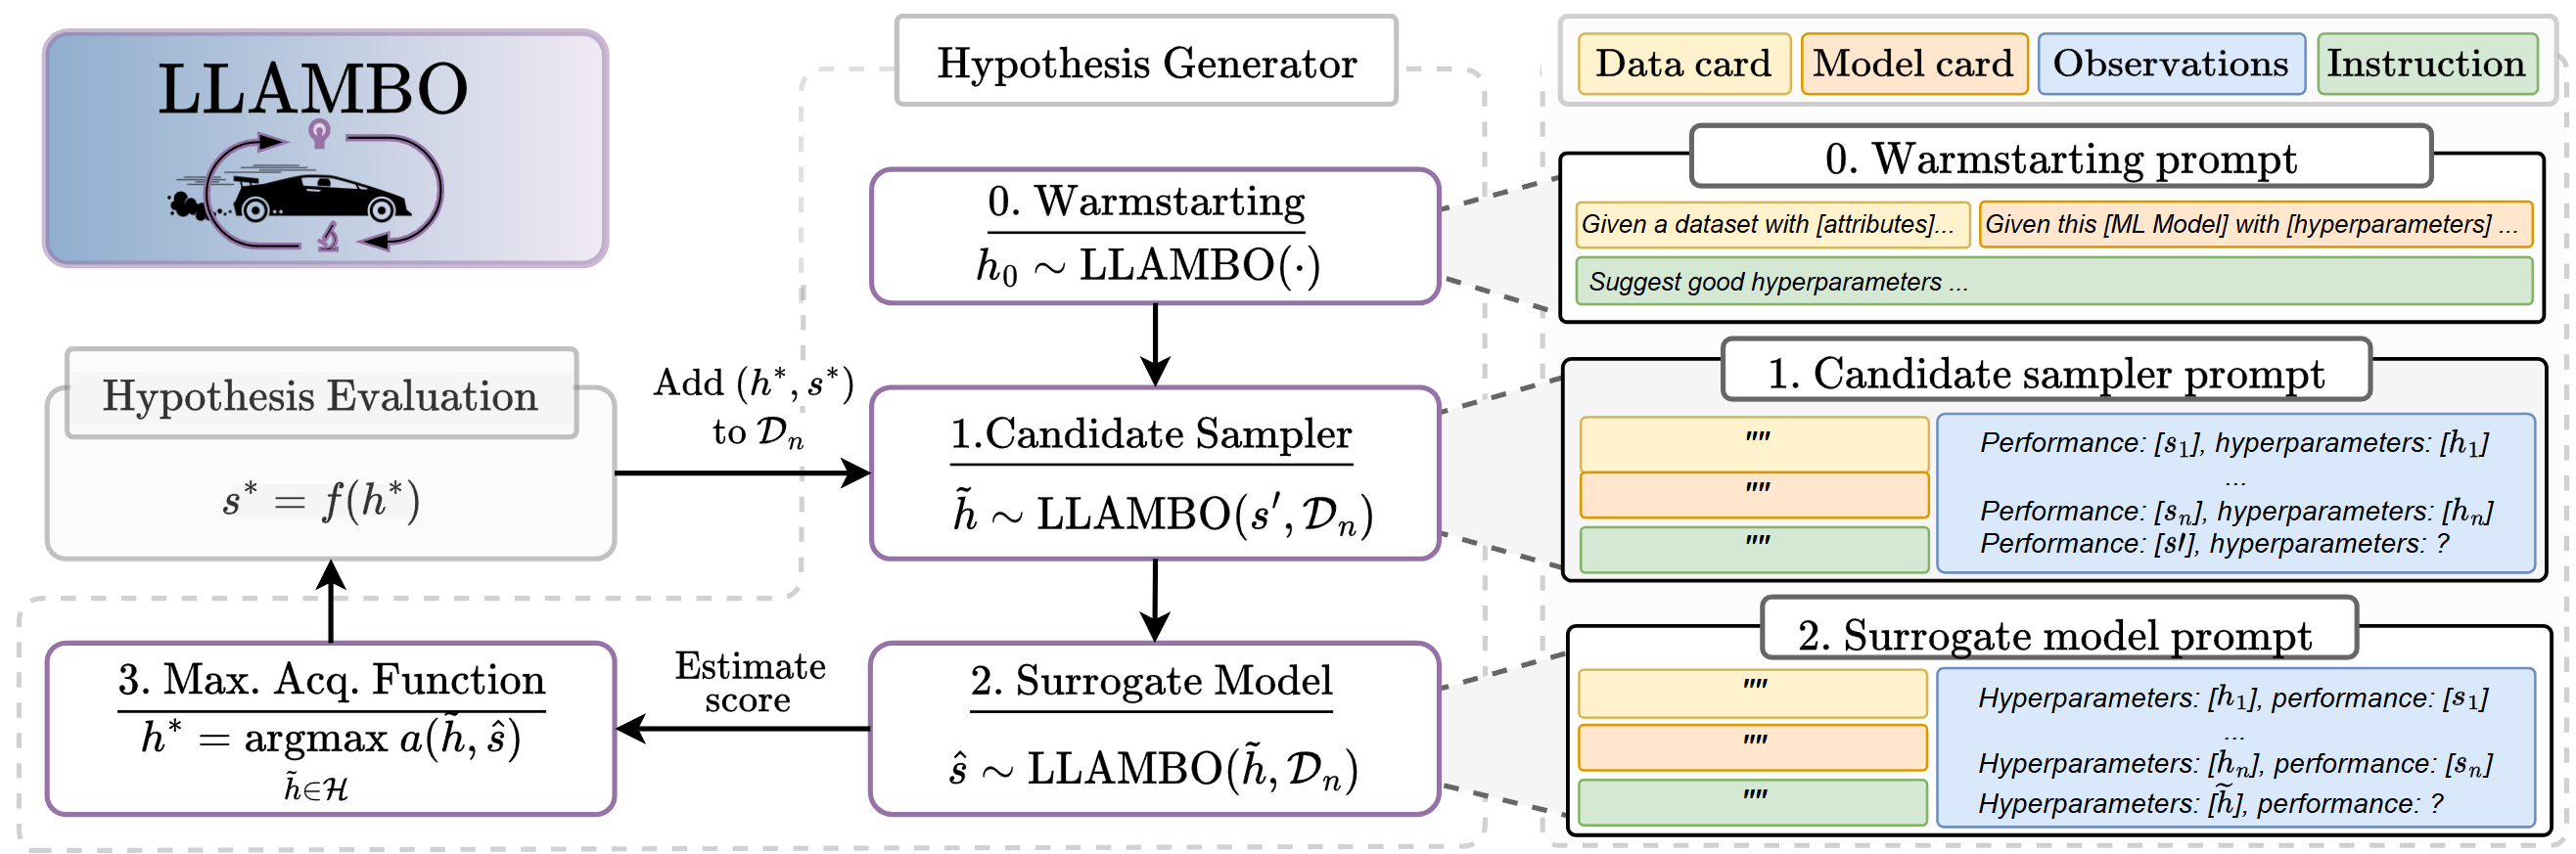
\includegraphics[width=1.0\textwidth]{images/llambo}

Translation of notation:
$s = \cost$ at a specific $\conf$, $f = \cost$ as a function, $h = \conf$
    
\end{frame}

\begin{frame}{LLINBO: Trustworthy Hybrid Framework \liturl{Chang et al. 2025}{https://arxiv.org/abs/2505.14756}}
    \begin{itemize}
        \item \textbf{Limitations of LLM-Assisted BO:} Pure LLM optimizers lack explicit calibrated uncertainty, and their effectiveness degrades as statistical surrogates accumulate data.
        \item \textbf{LLINBO Approach:} Combines LLMs for early-stage contextual exploration with Gaussian Processes (GPs) for principled exploitation.
        \item The statistical surrogate identifies optimal regions by maximizing an acquisition function, such as Upper Confidence Bound (UCB)
        \item The framework then uses one of three mechanisms to safely integrate or reject the LLM's suggested point, $\conf_{LLM,t}$.
    \end{itemize}
\end{frame}

\begin{frame}{LLINBO: Hybrid Framework \liturl{Chang et al. 2025}{https://arxiv.org/abs/2505.14756}}

    \centering
    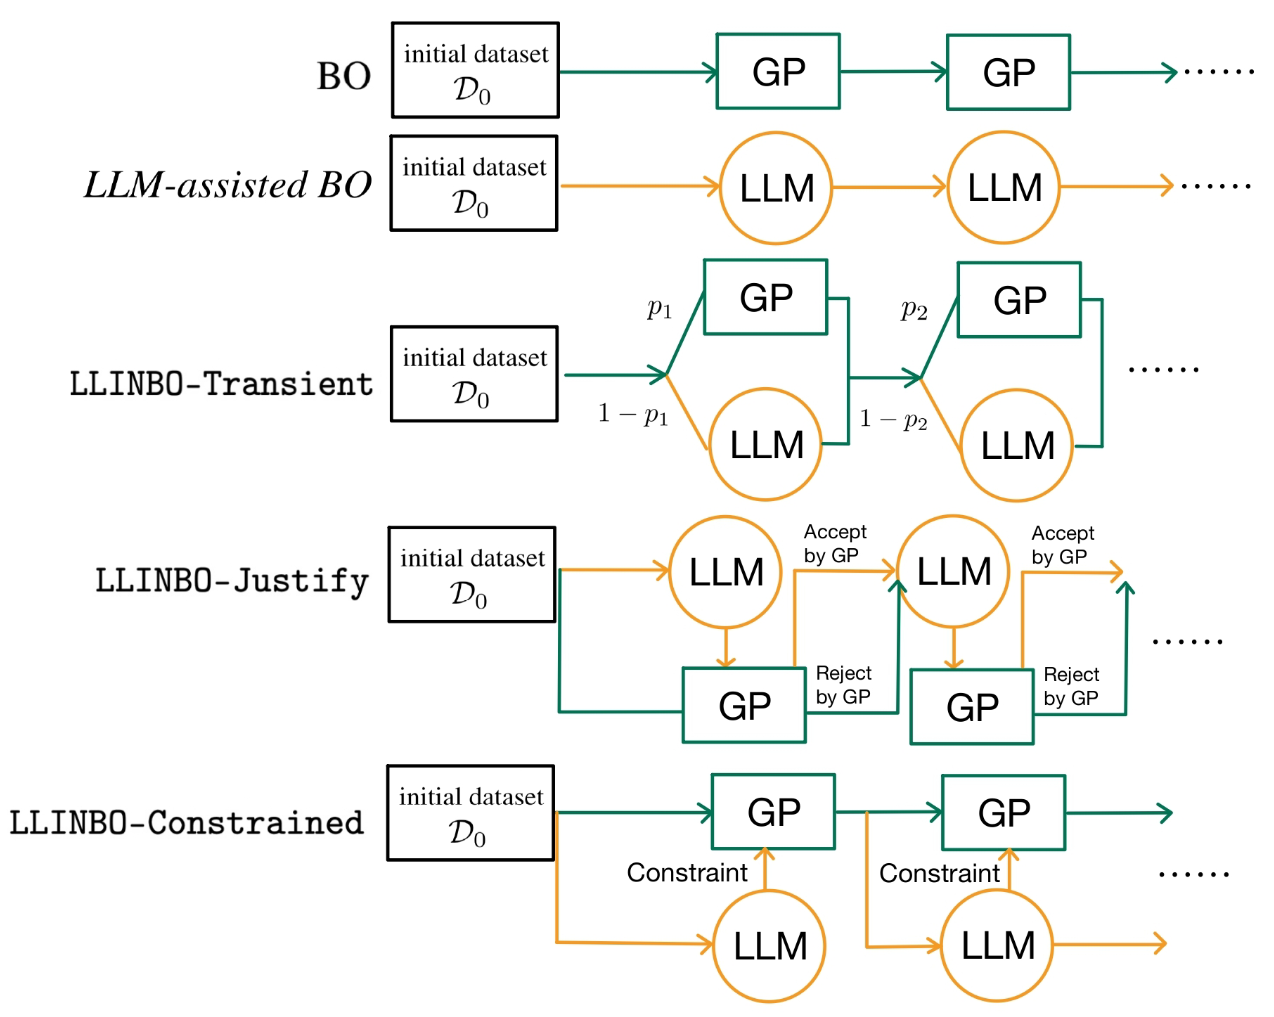
\includegraphics[width=0.58\textwidth]{images/llinbo.png}
\end{frame}

\begin{frame}{LLINBO-Transient Mechanism  \liturl{Chang et al. 2025}{https://arxiv.org/abs/2505.14756}}
    \begin{itemize}
        \item \textbf{Concept:} A probabilistic transition from LLM-guided exploration to GP-guided exploitation.
        \item \textbf{Selection Rule:} The query design $\conf_t$ is chosen as:
        \begin{equation*}
            \conf_t = 
            \begin{cases} 
            \conf_{GP,t} & \text{with probability } p_t \\ 
            \conf_{LLM,t} & \text{with probability } 1 - p_t 
            \end{cases}
        \end{equation*}
        \item $p_t$ is a monotonically increasing sequence (e.g., $1 - 1/t^2$) that approaches $1$ as iterations progress.
        \item Ensures that reliance on LLM suggestions diminishes as the statistical surrogate becomes better calibrated over time.
    \end{itemize}
\end{frame}

\begin{frame}{LLINBO-Justify and LLINBO-Constrained  \liturl{Chang et al. 2025}{https://arxiv.org/abs/2505.14756}}
    \begin{itemize}
        \item \textbf{LLINBO-Justify:} Uses the GP's acquisition function to validate the LLM's suggestion. It rejects $\conf_{LLM,t}$ if it is substantially worse than the GP's optimum:
        \begin{equation*}
            \alpha_{UCB}(\conf_{LLM,t}) \le \max_{\conf} \alpha_{UCB}(\conf) - \psi_t
        \end{equation*}
        \item \textbf{LLINBO-Constrained:} Treats the LLM suggestion as a potentially optimal design and refines the GP posterior via a constraint:
        \begin{equation*}
            \mathcal{GP}(\hist_{,t-1}) | \{\cost(\conf_{LLM,t}) > \max_{\conf} \mu_{t-1}(\conf)\}
        \end{equation*}
        \item Utilizes rejection sampling to dynamically accept the LLM's suggestion only if it aligns with the updated posterior support.
    \end{itemize}
\end{frame}


\begin{frame}{Main Takeaways}
    \begin{itemize}
        \item \textbf{Context accelerates search:} Utilizing textual problem descriptions and meta-data allows optimizers to fast-track early exploration in low-data regimes.
        \item \textbf{Uncertainty calibration is essential:} Purely generative or text-based optimizers struggle with rigorous uncertainty quantification, limiting their long-term convergence guarantees.
        \item \textbf{Hybrid synergy is optimal:} Integrating heuristic or context-driven priors with traditional statistical models leverages the early-stage strengths of the former and the asymptotic reliability of the latter.
        \item \textbf{Trust requires verification:} External or heuristic suggestions should not be blindly accepted; they must be verified or bounded by empirical observations and mathematical frameworks.
    \end{itemize}
\end{frame}


\end{document}

